\chapter{Calendrier annuel}
Ci-dessous vous trouverez un calendrier qui détaille les tâches que j'ai accompli entre le 25 septembre 2010 et le 14 septembre 2011.

~

\subsubsection{Légende}
\begin{description}
	\item[Gris (tous) :] périodes hors calendrier ou n'appartenant pas à l'année de mon alternance.
	\item[Rouge - Orange :] projet tuteuré.
	\item[Jaune pâle :] semaines de la formation à l'IUT A.
	\item[Bleu :] gestion des PDF.
	\item[Vert :] tâches annexes (non détaillé).
	\item[Jaune :] jours de congés.
	\item[Violet :] module de gestion commerciale pour les entrepôts.
	\item[Blanc : ] Tampon-FLASH.
\end{description}

\begin{figure}[h!]
	\begin{center}
		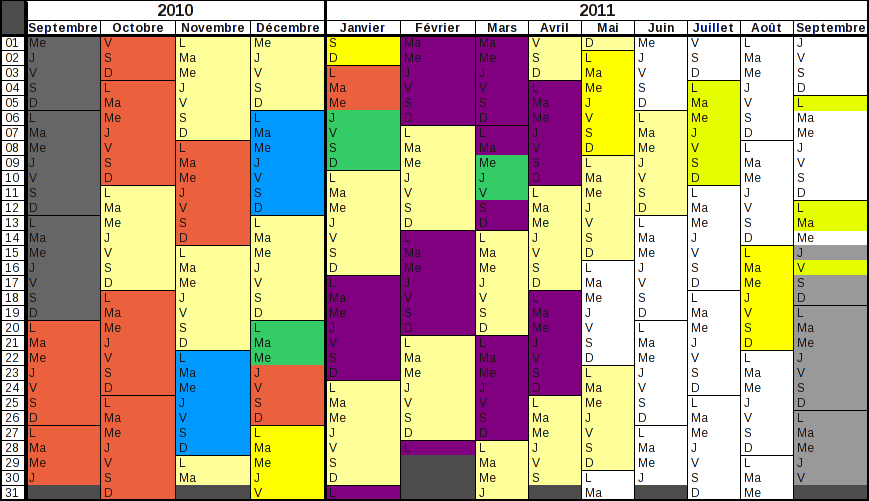
\includegraphics[scale=1, angle=90]{Contenu/Annexes/Images/Calendrier.png}
	\end{center}

	\caption{Calendrier des tâches effectuée pendant mon alternance}
	\label{calendrier}
\end{figure}
